\documentclass[journal]{IEEEtran}
\usepackage{amsmath,amssymb}
\usepackage{graphicx}
\usepackage{booktabs}
\usepackage{cite}
\usepackage[hidelinks]{hyperref}
\graphicspath{{figs/}}

\newcommand{\rzero}{r_0}
\newcommand{\tauc}{\tau_{\mathrm{corr}}}

\begin{document}

\title{Overclocking the p-bit: Stochastic Binary Neural Network Inference
with Autocorrelated sMTJ Randomness}

\author{Manan~Gupta%
\thanks{M.~Gupta is with The Harker School, San Jose, CA, USA
(e-mail: mnn@yogins.com).}}

\maketitle

\begin{abstract}
Stochastic magnetic tunnel junctions (sMTJs) supply physically random bits
at $\sim$0.03\,pJ per bit, roughly six orders of magnitude below software
pseudorandom generation, making them natural entropy sources for
probabilistic-bit (p-bit) neural hardware. A standard design rule requires
sampling an sMTJ no faster than twice its mean dwell time so that
successive bits are uncorrelated; existing systems obey it by construction,
and its cost to an application has not been measured. Treating the
sampling-to-correlation-time ratio as a continuous design knob, we simulate
stochastic binary network classification on MNIST and Fashion-MNIST with
telegraph-process sMTJ neurons and measure where accuracy actually fails.
Operating mode, not sampling rate, is decisive. With a per-input settle of
$\approx 4$ correlation times---a requirement we measure, not
assume---accuracy is nearly rate-independent: $200\times$ faster-than-rule
sampling costs under 0.7 accuracy points. In continuous streaming
operation, stale device state carries each input's activations into the
next, and single-sample accuracy collapses to chance. Device-to-device
dwell-time dispersion can either harm or \emph{rescue} streaming accuracy,
depending on whether it adds slow or fast devices: a single
effective-refresh parameter, dominated by the fast quantile of the device
population, approximately predicts accuracy across all dispersion models.
Finally, correlation-aware training---backpropagating while activations are
sampled from the correlated process---recovers most of the streaming loss
(28\%$\to$86\% at the harshest operating point), extending the
accuracy--throughput Pareto frontier to $2\times$ the rule-compliant
optimum at 97\% accuracy, $4\times$ at 95\%, and $8\times$ at 90\%.
\end{abstract}

\begin{IEEEkeywords}
probabilistic computing, p-bit, stochastic magnetic tunnel junction,
binarized neural networks, random telegraph noise, energy-efficient inference
\end{IEEEkeywords}

\section{Introduction}
\IEEEPARstart{G}{enerating} randomness is expensive on conventional
hardware: pseudorandom generation at Gb/s rates costs $\sim$30\,nJ per bit
on CPUs and $\sim$3\,nJ per bit on GPUs~\cite{sun2026superparamagnetic}. A
stochastic magnetic tunnel junction (sMTJ)---a nanomagnet whose free layer
flips between two states under thermal agitation---delivers physically
random bits at $\sim$0.03\,pJ per bit~\cite{sun2026superparamagnetic}. This
$\sim$$10^6$ gap motivates probabilistic-bit (p-bit)
computing~\cite{camsari2017stochastic,kaiser2021probabilistic}, in which the
sMTJ is not a peripheral generator but the stochastic neuron itself: biased
by an input current, its time-averaged state follows
$\langle m \rangle = \tanh(I)$~\cite{camsari2017stochastic}---the
activation of stochastic binary neural networks (SBNNs).

Every physical entropy source has a clock. An sMTJ flips on its own
schedule; read faster than it flips, it returns copies of a stale state
rather than fresh samples. Daniels \emph{et al.}\ showed that the
autocorrelation between adjacent samples vanishes once the sampling
interval exceeds about twice the \emph{mean dwell time}
$\tau_d$~\cite{daniels2020energy}, and this ``$2\tau$ rule'' functions as a
hard constraint: system demonstrations oversample device relaxation times
by large factors~\cite{singh2024cmos}, and randomness quality is certified
by statistical suites that presume i.i.d.\
sampling~\cite{vodenicarevic2017low,sun2026superparamagnetic}. The
clock-versus-device-timescale trade has been characterized for sampling
machines: autonomous Ising-machine operation requires synapse response
faster than neuron fluctuation~\cite{sutton2020autonomous}, and in situ
Boltzmann learning requires the learning time constant to exceed the MTJ
fluctuation time~\cite{kaiser2022hardware}. What is missing is the
\emph{application-side price curve}: no published work maps the sampling
ratio continuously onto feedforward classification accuracy, distinguishes
the operating modes in which that price is or is not paid, or asks what
training can buy back. This paper does. Concretely, our contributions are:

\begin{itemize}
\item \textbf{Mode, not rate, is decisive.} We simulate sMTJ neurons as
input-biased telegraph processes (exact discrete-time propagator;
stationary law equal to the p-bit activation) and sweep the sampling ratio
$\rzero = \Delta t/\tauc(0)$ across four decades. With a per-input settle
of $\approx 4\tauc$---a requirement we \emph{measure} by sweeping the
settle interval, replacing the folklore idle assumption---classification is
nearly rate-independent: at $\rzero = 0.02$, i.e.\ $200\times$ past the
rule, 32-sample accuracy drops only $97.7\%\to97.1\%$. In continuous
streaming operation, stale state leaks each input's activations into the
next input's samples and single-sample accuracy collapses to chance
(10\%) below $\rzero \approx 0.1$; sample-averaging buys roughly a decade.
The collapse persists (indeed worsens) under a bias-independent-rate
device variant, so it is generic staleness, not an artifact of the
Arrhenius parameterization.
\item \textbf{The fast quantile governs variability.} Whether
device-to-device dwell-time dispersion hurts or helps streaming depends
entirely on which population statistic fabrication holds fixed: with the
median device fixed, dispersion adds a slow tail and degrades accuracy;
with the mean correlation time fixed, dispersion adds fast devices and
\emph{rescues} accuracy ($72\%\to94\%$ at $\rzero=0.05$,
$\sigma_\Delta = 1.5\,k_BT$). A single effective-refresh parameter
$\mathbb{E}[1-e^{-\Delta t/\tau}]$ approximately collapses both regimes,
identifying the fast quantile of the device population---not its mean or
slow tail---as the quantity a device specification should target.
\item \textbf{Correlation-aware training extends the Pareto frontier.}
Training while activations are sampled from the same correlated telegraph
process (state running continuously across minibatches) recovers most of
the streaming loss: $28\%\to86\%$ at $\rzero=0.02$ ($T{=}32$), at a
1--3 point cost at nominal speed. With physically-accounted throughput
(settle mode pays its measured $\approx 4\tauc$ per input), the
accuracy--throughput frontier reaches $2\times$ the best rule-compliant
operating point at 97\% accuracy, $4\times$ at 95\%, and $8\times$ at
90\%---the latter two from training alone.
\end{itemize}

\section{Background and Related Work}
\label{sec:related}

\subsection{p-bits and sMTJ entropy sources}
A p-bit outputs $m = \mathrm{sgn}\{\mathrm{rand}(-1,1) + \tanh I\}$ per
query, so $\langle m \rangle = \tanh(I)$~\cite{camsari2017stochastic};
superparamagnetic MTJs with barriers near
$1.4\,k_BT$~\cite{sun2026superparamagnetic} realize this natively, with
dwell times $\tau = \tau_0 e^{\Delta/k_BT}$,
$\tau_0 \approx 10\,\mathrm{ps}$--$1\,\mathrm{ns}$
\cite{camsari2017stochastic}. Demonstrated fluctuation timescales span
nanoseconds---2--5\,ns autocorrelation in easy-plane
devices~\cite{safranski2021nanosecond}, ns-scale telegraph noise in
in-plane junctions~\cite{hayakawa2021nanosecond}---to the
microsecond-and-slower devices of early p-bit
demonstrations~\cite{borders2019integer}, whose system used
$\sim$ms-class fluctuations; a recent heterogeneous
CMOS-plus-nanomagnet system oversamples its $\sim$20\,ms relaxation by
$40\times$~\cite{singh2024cmos}.

\subsection{Randomness quality, sampling, and neural inference}
Robustness studies of MTJ neural hardware concentrate on \emph{static}
imperfections: process-variation-induced sigmoid
distortion~\cite{wood2020modular,zand2018composable} and fabricated-array
parameter spread with compensation~\cite{zhang2025automatic}. sMTJ
generators are validated with NIST statistical
suites~\cite{vodenicarevic2017low,sun2026superparamagnetic}; software-PRNG
quality shows a threshold effect on MNIST
training~\cite{prng2025quality}; measured sMTJ bitstreams have driven
stochastic-computing inference with whatever correlation the apparatus
had~\cite{spintronicSC2025}. The stochastic-computing literature has long
recognized bit-level correlation as a first-order design
variable~\cite{alaghi2013survey,alaghi2013exploiting}, and multi-sample
averaging of stochastic binary activations---including training through
the average---was recently shown to improve p-bit network
accuracy~\cite{ghantasala2026sampling}. On the theory side, the cost of
correlated samples is classical: autocorrelation time divides the
effective sample size of any Monte Carlo average~\cite{sokal1997monte},
and noise level has a computational optimum in spiking
networks~\cite{timcheck2022optimal}. Our contribution sits at the
unoccupied intersection: the sampling ratio as a continuously swept
variable, mapped to feedforward classification accuracy, across operating
modes, device-variability models, and training regimes.

\section{Model}
\label{sec:model}

\subsection{The sMTJ neuron as a biased telegraph process}
Each hidden unit is a two-state fluctuator $s \in \{-1,+1\}$ with
input-modulated Arrhenius escape rates
\begin{equation}
k_{-\to+} = f\, e^{+I}, \qquad k_{+\to-} = f\, e^{-I},
\label{eq:rates}
\end{equation}
where $I$ is the dimensionless synaptic input and $f = f_0 e^{-\delta
\Delta}$ the device attempt rate with per-device barrier offset
$\delta\Delta$ (in $k_BT$). The stationary law is
\begin{equation}
P(s{=}{+}1) = \frac{k_{-\to+}}{k_{-\to+}+k_{+\to-}} = \frac{1+\tanh I}{2}
\equiv p,
\label{eq:peq}
\end{equation}
which follows from $\langle m\rangle = \tanh I$
\cite{camsari2017stochastic} since $\langle m\rangle = 2P(+1)-1$: the mean
behavior of every neuron is exactly the p-bit activation at every
operating point; only the time structure changes. The correlation time is
\begin{equation}
\tauc(I) = \frac{1}{k_{-\to+}+k_{+\to-}} = \frac{1}{2f\cosh I},
\label{eq:tauc}
\end{equation}
so saturated neurons decorrelate faster. Note the distinction between
$\tauc$ and the mean dwell time: at $I{=}0$, $\tau_d = 1/f = 2\tauc$, so
the Daniels $2\tau_d$ rule~\cite{daniels2020energy} corresponds to
$\rzero \geq 4$ in our units,
\begin{equation}
\rzero \;=\; 2 f_0 \Delta t \;=\; \Delta t/\tauc(0)\big|_{\delta\Delta=0}.
\end{equation}
Under the assumption that inputs are piecewise-constant over each
inter-query interval (sample-and-hold operation between clocked layers),
the exact two-state propagator applies with no discretization error:
\begin{equation}
P(s_{t+\Delta t}{=}{+}1 \mid s_t) = p + \left(\mathbb{1}[s_t{=}{+}1] -
p\right) e^{-\Delta t/\tauc},
\label{eq:propagator}
\end{equation}
with $\Delta t/\tauc = \rzero e^{-\delta\Delta}\cosh I$.

Eq.~\eqref{eq:rates} is the energy-tilt picture appropriate for
barrier-type (Arrhenius-regime) devices. Easy-plane sMTJs are engineered
so the fluctuation rate is only weakly
bias-dependent~\cite{safranski2021nanosecond,sun2026superparamagnetic};
we therefore also simulate a \textbf{bias-independent-rate variant}
(total rate fixed at $2f$, giving $\Delta t/\tauc = \rzero
e^{-\delta\Delta}$ with the same stationary law), and report where the two
device classes differ. Device variability is modeled as $\delta\Delta \sim
\mathcal{N}(\mu, \sigma_\Delta^2)$ fixed per chip. Because dwell time is
exponential in $\delta\Delta$, the choice of $\mu$ decides which
population statistic is held fixed as $\sigma_\Delta$ grows:
$\mu = 0$ fixes the \emph{median} device (the mean correlation time then
grows as $e^{\sigma_\Delta^2/2}$), while $\mu = -\sigma_\Delta^2/2$ fixes
the \emph{mean} correlation time. We simulate both, since real
fabrication corners could resemble either. In both cases every stationary
firing probability is untouched, isolating the purely temporal effect of
variability, complementary to static sigmoid-distortion
studies~\cite{wood2020modular,zand2018composable,zhang2025automatic}.
Idealizations: no read-disturb, no $1/f$ resistance noise, no
temperature drift, two-state
telegraph regime~\cite{safranski2021nanosecond,hayakawa2021nanosecond}.

\subsection{Operating modes: settle vs.\ streaming}
\label{sec:modes}
In \textbf{settle mode} (batch-style inference), the input is applied and
the device relaxes for an interval $t_s = \rho\,\tauc(0)$ before the first
of $T$ reads taken $\Delta t$ apart. Physically, an idle device
equilibrates to $p = 1/2$, \emph{not} to the upcoming input's stationary
law; the settle relaxes it toward $p_{\mathrm{eq}}(I)$ with the same time
constant $\tauc(I)$, so the first read carries a residual bias
$\propto e^{-\rho \cosh I}$. We simulate this relaxation explicitly---the
settle is a propagator step from the device's actual prior state---and
sweep $\rho$ to find the requirement empirically. Throughput accounting
charges $\rho$ per input: settle-mode throughput is
$1/(T \rzero + \rho)$ images per $\tauc$, bounded by $1/\rho$ however fast
the reads are. In \textbf{streaming mode} the devices are never idle:
state persists from each input to the next (throughput $1/(T\rzero)$).
In the limit of perfect settling ($\rho \to \infty$), a single settle-mode
read per input is a draw from the stationary law
Eq.~\eqref{eq:peq}---single-shot accuracy is then exactly
rate-independent, a useful simulator sanity check rather than a deep
result; the empirical question, answered below, is how large $\rho$ must
be and what the $T$ correlated reads cost.

\subsection{Network and training}
We use a $784{-}256{-}128{-}10$ MLP with stochastic bipolar hidden
activations resampled at every query \emph{including inference} (p-bit
operating style, unlike test-time-deterministic binarized
networks~\cite{courbariaux2015binaryconnect,hubara2016binarized});
real-valued input and readout layers follow standard practice. Class
scores average $T$ stochastic passes. Baselines train with ideal i.i.d.\
randomness and a straight-through
estimator~\cite{bengio2013estimating}; correlation-aware networks train
identically but with hidden activations sampled from the telegraph model,
device state running continuously across minibatches.

\section{Experimental Setup}
\label{sec:setup}
Datasets: MNIST~\cite{lecun1998gradient} with Fashion-MNIST
\cite{xiao2017fashion} replication. The last 5{,}000 training images form
a validation split used for all model selection; the 10{,}000-image test
set is used only for reported numbers. Training: 30 epochs, Adam
($10^{-3}$, cosine decay); ideal-randomness anchors reach $97.0\%$
($T{=}1$) and $97.8\%$ ($T{=}32$) on MNIST. Sweeps cover $\rzero \in
[0.02, 10]$ and $T \in \{1,\dots,64\}$ with 3--5 thermal seeds per point
(binomial SE on the 10k test set is $\pm0.2$--$0.5$ points; error bars
report seed std). Baseline findings replicate across five independently
trained networks; correlation-aware results average three training seeds
per configuration (except $\rzero^{\mathrm{train}}{=}0.1$, one seed).
Streaming is evaluated as true per-lane sequential streams: the test set
is split into 100--200 independent lanes, each preceded by unscored
warm-up images from the training pool so that scored images are in steady
state; measured accuracy is invariant to lane count (72.3\%, 72.1\%,
71.7\%, 72.3\% at 50/100/200/500 lanes for the same operating point),
confirming the protocol. Every result file records its git revision, and
runs are reused only when revisions match. The simulator's stationary
law, autocorrelation decay at zero and nonzero bias, settle-relaxation
distribution, and variant behaviors are validated by unit tests against
Eqs.~\eqref{eq:peq}--\eqref{eq:propagator}. All experiments run on CPU in
hours; code, per-run records, and configurations are in the project
repository, public upon publication.

\section{Results}
\label{sec:results}

\begin{figure}[t]
\centering

\includegraphics[width=\columnwidth]{fig_model}
\caption{Telegraph sMTJ neuron at three sampling ratios, driven by a
slowly varying firing probability (dashed). At $\rzero{=}10$ samples are
effectively i.i.d.; at $\rzero{=}0.05$ the device returns long runs of
stale state.}
\label{fig:model}
\end{figure}

\begin{figure*}[t]
\centering
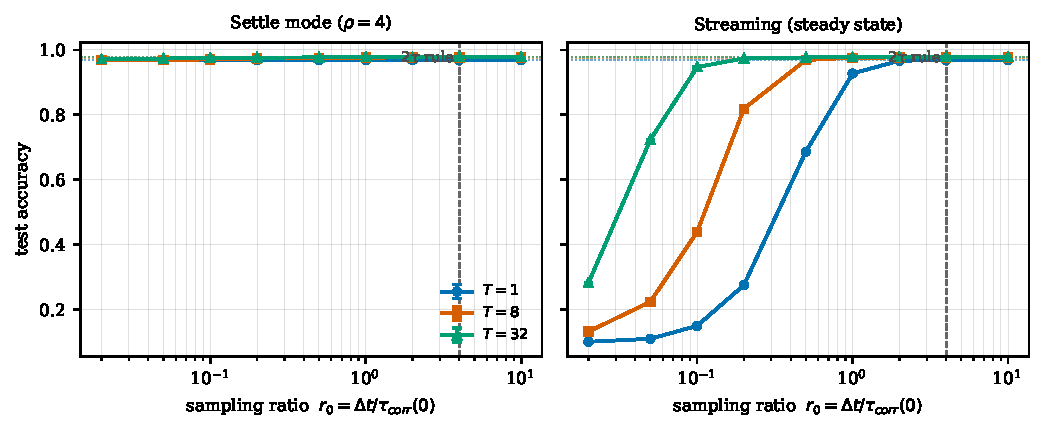
\includegraphics[width=0.9\textwidth]{fig_e2_correlation}
\caption{Accuracy vs.\ sampling ratio $\rzero$ (MNIST; mean $\pm$ std
over thermal seeds; dotted: ideal-randomness anchors; dashed vertical:
the $2\tau_d$ rule, $\rzero = 4$). \textbf{Left:} settle mode
($\rho{=}4$) is nearly rate-independent. \textbf{Right:} steady-state
streaming collapses; $T{=}1$ reaches chance below $\rzero \approx 0.1$.}
\label{fig:e2}
\end{figure*}

\subsection{Mode, not rate (E2)}
Fig.~\ref{fig:e2} is the central result. \textbf{Settle mode:} with
$\rho = 4$, single-read accuracy is flat at $96.90\%$ across the entire
sweep, and $T{=}32$ accuracy falls only $97.73\%\to97.12\%$ at
$\rzero{=}0.02$---$200\times$ past the rule. The settle sweep locates the
actual re-equilibration requirement: at $\rzero{=}0.02$, $T{=}1$ accuracy
is $92.9\%$, $96.6\%$, $96.9\%$, $96.8\%$ for $\rho = 1, 2, 4, 8$---a
settle of $\approx 4\tauc$ suffices and $\approx 1\tauc$ measurably does
not. The residual $T{=}32$ loss is the effective-sample-size cost of
correlated averaging~\cite{sokal1997monte}: stale within-input reads
shrink $T$ toward an effective $T_{\mathrm{eff}}$, and the floor---the
$T{=}1$ anchor---is high.

\textbf{Streaming:} steady-state accuracy collapses, and far harder than
a warm-start-contaminated protocol would suggest. Single-shot accuracy is
$96.7\%$ at $\rzero{=}2$, $92.7\%$ at $1$, $68.6\%$ at $0.5$, $27.5\%$ at
$0.2$, and chance ($\approx 10\%$) at $\rzero \leq 0.1$: each input
inherits the previous input's activation pattern through the device
state. Averaging buys roughly a decade per $\sim$$16\times$ increase in
$T$ (90\%-crossings at $\rzero \approx 0.9, 0.35, 0.13$ for
$T = 1, 8, 32$), but at $\rzero = 0.02$ even $T{=}32$ retains only
$28.1\%$. The same qualitative structure holds for the
bias-independent-rate variant---collapse thresholds shift roughly
$2$--$4\times$ \emph{higher} ($T{=}32$ falls to $53.8\%$ already at
$\rzero{=}0.1$, vs.\ $94.7\%$ for the Arrhenius device)---showing (i) the
collapse is generic staleness, not a parameterization artifact, and (ii)
the input-dependent rate boost $\cosh I$ of barrier-type devices is
\emph{protective}: strongly driven neurons refresh fastest exactly where
it matters. Fashion-MNIST reproduces the full pattern: settle-mode $T{=}32$ falls
only $88.1\%\to87.0\%$ at $\rzero{=}0.02$, while steady-state streaming
falls to $30.2\%$ ($T{=}32$) and to chance ($T{=}1$).

\begin{figure*}[t]
\centering

\includegraphics[width=0.9\textwidth]{fig_e3_hetero}
\caption{\textbf{Left:} whether dwell-time dispersion hurts or rescues
streaming depends on the fixed population statistic: median-fixed
(solid) adds a slow tail and degrades; mean-$\tauc$-fixed (dashed) adds
fast devices and rescues ($T{=}32$, 5 chips, streaming). \textbf{Right:}
a single effective-refresh parameter approximately collapses all cells.}
\label{fig:e3}
\end{figure*}

\subsection{The fast quantile governs variability (E3)}
Because dwell time is exponential in the barrier offset, ``add
dispersion'' is ambiguous until one says which statistic is held fixed.
Fig.~\ref{fig:e3} (left) shows both fabrication corners at fixed
$\rzero$: with the \emph{median} device fixed, dispersion grows the slow
tail (and the mean correlation time, by Jensen's inequality) and accuracy
degrades ($72.0\%\to67.5\%$ at $\rzero{=}0.05$,
$\sigma_\Delta{:}\,0\to1.5$); with the \emph{mean} correlation time
fixed, the same dispersion supplies a fast sub-population and accuracy
\emph{rises} dramatically ($72.0\%\to94.4\%$). The two corners are
reconciled by a single scalar: the population-averaged per-query refresh
$\mathbb{E}_{\delta\Delta}[1-e^{-\Delta t/\tau}]$, which approximately
collapses every $(\rzero, \sigma_\Delta, \mathrm{centering})$ cell onto
one curve (Fig.~\ref{fig:e3}, right). The engineering reading inverts
the usual uniformity discussion~\cite{zhang2025automatic}: for
overclocked streaming operation, what matters is not tight uniformity per
se but the \emph{fast quantile} of the dwell-time distribution---a few
fast devices per layer carry the network.

\begin{figure}[t]
\centering

\includegraphics[width=\columnwidth]{fig_e4_training}
\caption{Correlation-aware training flattens the streaming failure curve
(steady-state, $T{=}32$; mean $\pm$ std over training and thermal
seeds).}
\label{fig:e4}
\end{figure}

\subsection{Correlation-aware training (E4)}
Networks trained with the telegraph source active learn representations
that survive staleness (Fig.~\ref{fig:e4}). At $T{=}32$ streaming, the
network trained at $\rzero^{\mathrm{train}}{=}0.2$ holds $84.6\%$ at
$\rzero{=}0.02$ where the ideal-trained baseline retains $28.1\%$---a
$+57$-point recovery costing $3.3$ points at nominal speed ($94.5\%$
vs.\ $97.8\%$); the $\rzero^{\mathrm{train}}{=}0.5$ network trades less
nominal accuracy ($96.6\%$) for a smaller deep-overclock rescue. At
$T{=}1$ the rescue is partial---$70.6\%$ vs.\ $27.5\%$ at
$\rzero{=}0.2$---so training and averaging compose rather than
substitute. This extends multi-sample (``sample-aware'')
training~\cite{ghantasala2026sampling} along the temporal axis: what is
learned here is robustness to \emph{correlation between} samples, not
benefit from their number.

\begin{figure}[t]
\centering

\includegraphics[width=\columnwidth]{fig_pareto}
\caption{Accuracy vs.\ physically-accounted throughput (settle mode pays
its measured $\rho{=}4$ per input; dashed vertical: best rule-compliant
single-read throughput $\rzero{=}4$). Correlation-aware points use
validation-selected training ratios.}
\label{fig:pareto}
\end{figure}

\subsection{Throughput and energy (E5)}
Settle-mode throughput is bounded by $1/\rho = 0.25$ images per $\tauc$
regardless of read speed; streaming has no such bound but pays the
collapse; correlation-aware training moves the streaming curve
(Fig.~\ref{fig:pareto}). Model selection for the correlation-aware
points uses the validation split only. Against the best rule-compliant
operating point at each accuracy target, the frontier reaches:
$2.0\times$ at $97\%$ (streaming $T{=}2$, $\rzero{=}2$: $97.3\%$),
$4.0\times$ at $95\%$ (correlation-aware single-shot streaming at
$\rzero{=}1$: $95.6\%$), and $8.0\times$ at $90\%$ (correlation-aware
single-shot at $\rzero{=}0.5$: $92.5\%$). These are threshold statements
on a finite grid---the conceded accuracy at the $90\%$ target is
$2.5$ points below the bar-clearing rule point---and they assume readout
electronics are not limiting. For a millisecond-class device
($\tauc \sim 10$\,ms), the rule-compliant optimum is $\sim$25
single-read classifications/s; the frontier makes $\sim$100/s available
at $\geq$95\% accuracy and $\sim$200/s at $\geq$90\% from the same
silicon. Randomness-generation energy follows the bit count
($384\,T$ bits/inference): at $T{=}32$, $0.37$\,nJ from sMTJs vs.\
$37$--$369\,\mu$J from GPU/CPU PRNGs at the verified per-bit
figures~\cite{sun2026superparamagnetic}---five to six orders of
magnitude, unchanged by $\rzero$; overclocking converts that energy
advantage into throughput rather than surrendering it to the $2\tau$
wait. An alternative decorrelation strategy---interleaving $k$ devices
per neuron round-robin---multiplies each device's effective sampling
interval by $k$, i.e.\ moves along the same accuracy-vs-$\rzero$ curves
at $k\times$ device area; our curves thus also quantify that
area-throughput trade.

\section{Discussion}
\label{sec:discussion}
\textbf{Design guidance.} (i) The $2\tau_d$ rule is the right
specification for TRNG bitstream
certification~\cite{vodenicarevic2017low,sun2026superparamagnetic}, but
for classification inference it is workload-dependent: batch-style
(settle-mode) pipelines can read devices essentially arbitrarily fast,
provided each input is given its $\approx 4\tauc$ settle---which becomes
the real throughput cost. (ii) Streaming pipelines face a genuine
boundary; it is moved by correlation-aware training and by sample
averaging, not by fabrication uniformity. (iii) If overclocked streaming
is the target, device populations should be specified by their fast
dwell-time quantile rather than their mean. (iv) Barrier-type
(Arrhenius) devices tolerate overclocking better than
bias-independent-rate devices at matched $\tauc$, because strong inputs
buy fast refresh exactly where decisions are made.

\textbf{Limitations.} This is a simulation study with an idealized
two-state model: no read-disturb, retention drift, or $1/f$ components
\cite{sun2026superparamagnetic}, small MLPs, and MNIST-class benchmarks.
Streaming results assume consecutive inputs are uncorrelated; correlated
input streams (e.g.\ video) could interact with staleness in either
direction. The Pareto gains are grid-limited threshold statements, not
continuous optima. Validation on fabricated arrays---e.g.\ the
instrumented systems of \cite{singh2024cmos}---and extension to
convolutional networks and temperature drift are natural next steps.

\section{Conclusion}
The price of violating the sMTJ sampling rule is not a wall but a fork.
Batch-style inference with a measured $\approx 4\tauc$ per-input settle
tolerates $200\times$ faster-than-rule sampling at under one accuracy
point; steady-state streaming collapses to chance, is governed by the
fast quantile of the device population, and is largely rescued by
correlation-aware training. Treating the sampling ratio as a design
variable converts device autocorrelation into usable throughput---up to
$2$--$8\times$ past the rule-compliant optimum depending on the accuracy
target---while keeping the $\sim$$10^6$ randomness-energy advantage that
motivates p-bit hardware in the first place.

\section*{Acknowledgments}
The author thanks the UCSB Summer Research Academy Track 1 instructors
for introducing him to probabilistic computing. AI tools (Anthropic
Claude) were used for literature search, simulation-code implementation,
experiment orchestration, and drafting/editing for accuracy and style;
the author directed the research questions, reviewed all analyses and
text, and takes responsibility for the content. An AI-assisted
adversarial review process was additionally used to stress-test the
methodology prior to submission.

\bibliographystyle{IEEEtran}
\bibliography{refs}

\end{document}
